%%%%%%%%%%%%%%%%%%%%%%%%%%%%%%%%%%%%%%%%%%%%%%%%%%%%%%


\section{Jet and Soft Functions in Soft-Collinear Effective Theory}
%https://arxiv.org/pdf/1410.1892.pdf

Below the factorization structure of the double differential jet production cross section is displayed in the context of Soft-Collinear Effective Theory, SCET, following the framework for inclusive jet production $pp \rightarrow jet + X$ developed in for jets of  %https://arxiv.org/abs/1801.00790

\begin{equation}
\frac{d \sigma}{ d p_{T} d m}=\sum_{a b c} f_{a}\left(x_{a}, \mu\right) \otimes f_{b}\left(x_{b}, \mu\right) \otimes H_{a b}^{c}\left(x_{a}, x_{b}, p_{T} / z, \mu\right) \otimes \mathcal{G}_{c}\left(z, p_{T} R, m, \mu, z_{\mathrm{cut}}, \beta\right)
\end{equation}
% equation from here https://arxiv.org/pdf/1811.06983.pdf



Image of factorization in this context

%SCET-factorization
~\cite{Becher:2014oda}
%https://arxiv.org/abs/1410.1892
\begin{figure}[htb]
\centering
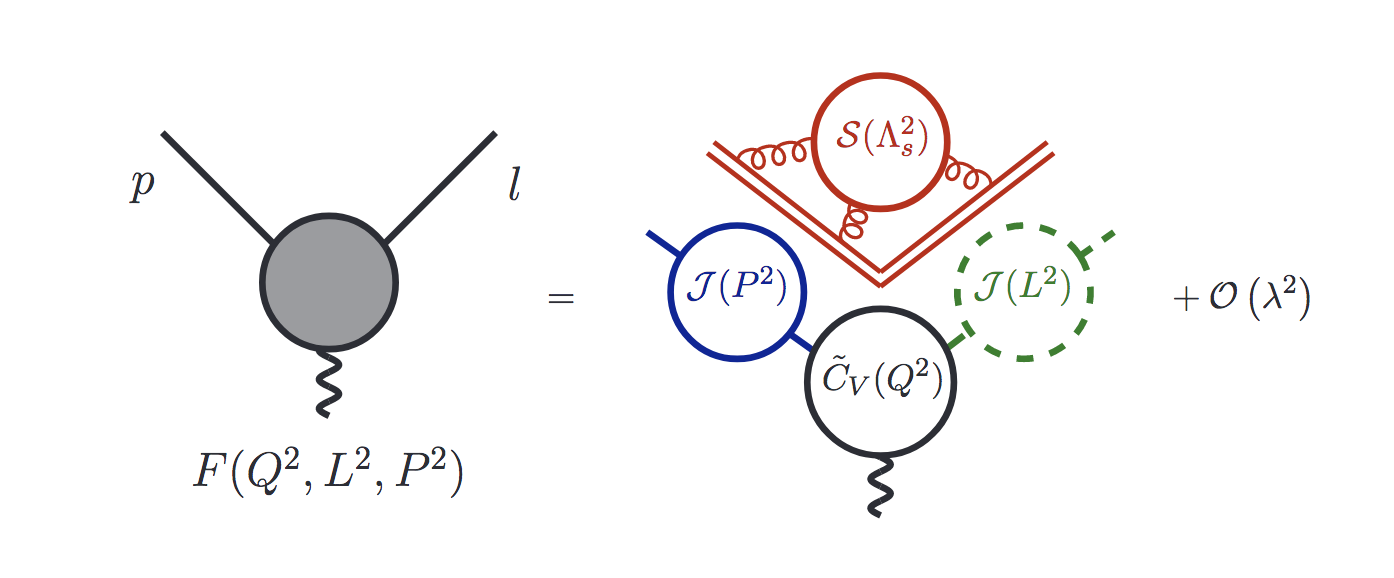
\includegraphics[width=1.0\textwidth]{visuals/SCET-factorization.png}
\caption{Fatorization of the energy scales in a hard scatter interaction according to SCET ~\cite{Becher:2014oda}.}
\label{fig:scet}
\end{figure}
discuss groomed jets in this context

comparing groomed  (Jet) to ungroomed (Jet+Soft)

\section{Jets Initited by Quarks and Gluons }\label{jetgroom:ch1}



earlier discussed $C_F = \frac{4}{3}$ and $C_A=3$ 

CITE A Theory of Quark vs. Gluon Discrimination
% https://arxiv.org/pdf/1906.01639.pdf

Dijets make quark gluon admixture %cite SMP-16-10
Z+Jets make mostly light quark jets, studied here and in 7 TeV analysis (1 D unfolding there and no soft drop)

% http://cms-results.web.cern.ch/cms-results/public-results/publications/SMP-16-010/index.html




% This similarity allows us to interpret the variations in quark enriched and gluon enriched jet samples in terms of the fundamental $C_F$ and adjoint $C_A$ casimirs, in $SU(3)$ ,   $C_F = \frac{4}{3}$ and $C_A=3$. 


%Comparing the probability of a quark to emit a gluon and that of a gluon to to emit a gluon we can see the ratio will give simply $\frac{C_A}{C_F} =\frac{9}{4} $. This has strong experimental implications since it implies gluon jets will on average be composed of about twice as many constituent particles as quark jets.



% ATLAS thesis http://inspirehep.net/record/1672323/files/2016_Mantifel_PhD_Atlas_Z.pdf



